\chapter{TRASH (IN) ART}




% Epigraph
\begin{singlespace}
\epigraph{One day, in a rubbish heap, I found an old bicycle seat lying beside a rusted handlebar, and my mind instantly linked them together. I assembled these two objects, which everyone then recognized as a bull’s head. The metamorphosis was accomplished, and I wish another metamorphosis would occur in the reverse sense. If my bull’s head were thrown in a junk heap, perhaps one day some boy would say, \quotes{Here’s something that would make a good handlebar for my bicycle!}}{\hfill ---Pablo Picasso, \textit{Trashformations}, 1998}
\end{singlespace}





In this chapter, questioned the purpose and meaning of using trash as a medium in the artworks. The reasons and motivations of artists who use trash are analyzed. The artist uses discarded items in their work is analyzed in the light of arguments discussed in the previous chapter. Questioned that why artists select to use society's debris rather than fresh items. Researched the place of trash in the world of art by looking at different methods and approaches. Started from masterpieces and founding works. Continued with recent examples of artworks.  

% Çöpün sanatta kullanılmasının temelleri arastirilmakta.

% Ben bölümde aslında çöpün sanatta nasıl yer aldığına bakıyor olacağım. İlk kim kullanmış nasıl kullanmış. Sonrasında hangi anlamlarda kullanılmış. 

Firstly looked at how artist started using objects that are not produced by artist and with the purpose of making art. Their works are notable and founding works that open new dimensions to reconsider objects and their meaning. Further, they extended the ways of art making and the language of art. Therefore, it is important to analyze Their intent and methods are analyzed (how?). In other words, looked at the foundation of using non-art objects in the art making. First examples are analyzed and how it evolved over time is explored. Questioned that how they affected successor artist.

Secondly looked at the some examples of contemporary works (or works from recent history). In particular, capture the current approaches on trash. Several methods and genres are explored. 

Lastly focused on the inspiring documentary of Agnes Varda, The Gleaners and I which provides a general picture of the subject.





%
%
\section{Root in the Art History}
Using trashed objects in making art can be examined with the entrance of non-art objects into the art. In other words, using objects in different scope beyond their intended purpose or intended meaning and function. Developing artworks not only painting but also using paper and other stuff by pasting (or juxtaposing) them together. (How using non-art objects affected art? Fragments) Using object apart from their proposed meaning is not a new thing, through the ages people used objects and tools for different purposes. However, it is not discussed in the context of fine art and not accepted method for art making.

From the beginning of 20th-century non-art, objects draw the attention of the artist. Development of art in this century evolved through this non-art objects (or these objects play significant role development of art trough time). They bring new dimension (or perception) to consider objects. Usage of these objects dramatically changed the way people look at art. In short, they introduced a new way of making art.

One of the remarkable change in the 20th-century art is the using unconventional materials in the making of paintings and sculptures, rather than the original (pure, fresh) materials produced with the purpose of art. These objects are not normally considered as art, often because they already have a non-art function. Possibly they are part of different disciplines and markets. Their place in the society and people's mind commonly have a different meaning. Beyond them, artists started to use them for their own purposes. Objects gain different meanings and usages with the hands of artists. (It is explained in the previous chapter that objects are not static and absolute. Objects can be used for new purposes even if they lost their meaning and value in the conventional system.)

They questioned the way of traditional (conventional) way of art making in every dimension. Their approach out of the previous methods. They are looking for the beyond of painting. With using different objects they break the pureness of artwork. It is not pure anymore, fragmented. Boundaries are pushed. Using non-art objects in the production of art challenges existing conventions of painting. 

Using non-art object can be considered as moving away from the purification of art \todo{ref req}. It is a composition of different fragments and pieces. Rather than the traditional way of painting on canvas they composed their work with the combination of various objects from different context. With this approach works can be examined in multi-dimensional context.

% (Peki neden sanatçılar bunu tercih ettiler, buhran neydi? Azıcık öncesindeki kıpırdanmaları anlatmak gerekli. Bu apayrı ve uzun bir konu. Ama değişmeler yavaş yavaş gelmeye başlamıştı. Neye karşıydı, ne getirdi. Sanatın var olan kalıplarını yıkıp yerine ne koydu? ronesanstan beri gercekligin temsili uzerine kurulan sanat ve estetik anlayis coktan sorgulanmaya baslamistir izlenimcilerle birlikte.)

Before the 20th-century, artists started to inquiry the existing methods and themes of previous periods. Modern artists experimented with new ways of seeing and with fresh ideas about the nature of materials and functions of art. Previously paintings are based on linear perspective and realistic style. Themes are often composed of religious and mythical narratives \todo{MOMA ref}. After the second half of the 19th-century, they started to abandon these themes and painting methods. For instance, in the works of impressionist paint brushstrokes can be easily identified, and themes are composed of everyday scenes. With Cezanne, the linear perspective started to question and later reached to its peak point with cubism. Cubism is developed with the collaboration of the Picasso and Braque. Besides, these two artists experimented non-traditional materials in their works for the first time in the scope of fine art. They continuously produced works with using different objects. They support each others art. They showed that an endless potential lay there. They collaborated with each other on the development of cubism and collage.

One of the keys to understanding the importance of Cubism, of Picasso and Braque, is to consider their actions and how unusual they were for the time. When Braque, and then Picasso placed industrially-produced objects ("low" commercial culture) into the realm of fine art ("high" culture) they acted as artistic iconoclasts (icon=image/clast=destroyer). \todo{ref}

% Sanat disi objenin kullanilmasi aslinda sanatin saflasmasininda disinda yer almaktadir. Saf oz bir sekilde kurulmasindan ziyade farkli seylerin parcalarin bir araya gelmesiyle birlikte kullanilmasi. Tabuların yıkılması. Sınırlarının aşılması. geleneksel anlamda tuvalin uzerine boya surmekten ziyade farkli teknikler denenmeye baslanmistir. 20yuzyilda geleneksel sanat tum boyutlariyla yeniden ele alinmistir. Resmin konusu, sergileme bicimleri, yenikikler gostermistir.

Collage originates from the French \textit{coller} is an artistic technique of applying manufactured, printed, or found materials, such as bits of newspaper, fabric, wallpaper, etc., to a panel or canvas, frequently in combination with painting. In about 1912–13 Pablo Picasso and Georges Braque extended this technique, combining fragments of paper, wood, linoleum, and newspapers with oil paint on canvas to form compositions. Pasting paper is not a new technique but using this it in the art making is a revolutionary movement in the  language of art \cite{waldman1992collage}. 

Collage was a major turning point in the evolution of Cubism, and therefore a major turning point in the whole evolution of modernist art in this century \cite{greenberg1984collage}. 

Similar to the collage, assamblage is produced by the incorporation of three-dimensional elements. In 1961, the exhibition "The Art of Assemblage" was featured at the New York Museum of Modern Art. William C Seitz, the curator of the exhibition, described assemblages as being made up of preformed natural or manufactured materials, objects, or fragments not intended as art materials. \todo{ref.}

%Who invented collage--Braque or Picasso--and when is still not settled. because of most of their early works are undated and unsigned. the question of priority is less important rather than 

One of the earliest and notable examples of collage is Picasso’s \quotes{Still Life with Chair Caning} (1912), in which a piece of oilcloth which is used as tablecloth or self coverings with an imitation chair caning design was pasted onto the painting. This work of Picasso also can be considered as first example of assemblage because of a rope was used to frame the picture. Picasso combined painting with already existing materials. He used real objects to represent instead of painting. As mentioned in the name of the work Picasso give clues of the parts of it. For instance the oval canvas\todo{canvas or oilcloth?} and the rope around it represent the table. Pasted chair caning signifies the chair within the table. On the table folded paper shadow represent newspaper. Further there is a cut out lemon painted onto the table. \paraphrase{The three letters above the scrap of cloth, "JOU," can be understood as both the beginning of the word "JOURNAL," alluding to the customary newspaper lying across the café table, and as the French verb meaning "to play." The new technique of collage allowed new possibilities of playfulness. This was a new way of making art; instead of painting a thing, you could stick whatever it was right onto the canvas.} 

% Greenberg
% The abiding effect is of a constant shuttling between surface and depth, in which the depicted flatness is "infected" by the undepicted. Rather than being deceived, the eye is puzzled; instead of seeing objects in space, it sees nothing more than--a picture.

% \comment{\textbf{Pablo Picasso} first publicly utilized the idea when he pasted a printed image of chair caning onto his painting titled Still Life with Chair Caning (1912).} 

\begin{figure}[h!]
  \centering
  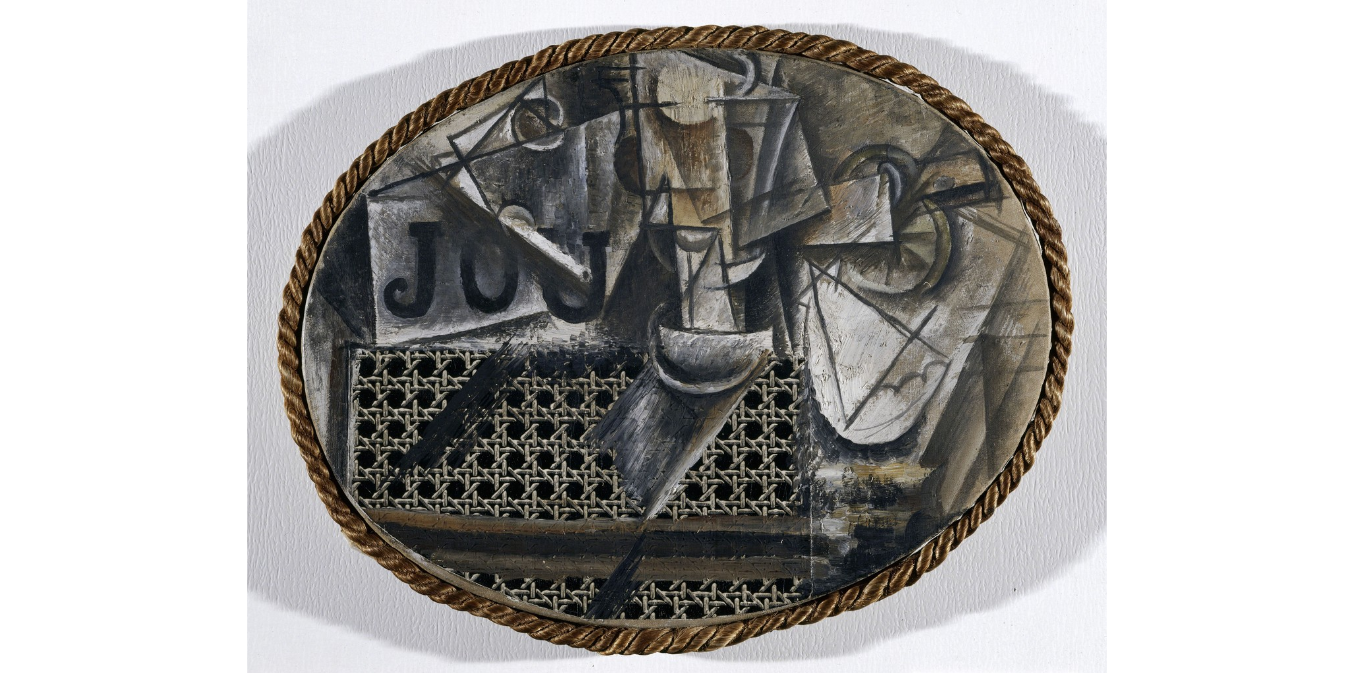
\includegraphics[height=6cm]{graphics/picasso_chair.png}
  \caption{Pablo Picasso, Still Life with Chair Caning, 1912, oil on oil-cloth over canvas edged with rope, 29 x 37 cm (Musée Picasso)}
  \label{fig:Picasso_Chair}
\end{figure}

Moreover, they questioned the elitism of the art world, which had always dictated the separation of common, everyday experience from the rarefied, contemplative realm of artistic creation. Of equal importance, their work highlighted and separated the role of technical skill from art-making. Braque and Picasso introduced a “fake” element on purpose, not to mislead or fool their audience, but rather to force a discussion of art and craft, of high and low, of unique and mass-produced objects. They ask: “Can this object still be art if I don’t actually render its forms myself, if the quality of the art is no longer directly tied to my technical skills or level of craftsmanship?"

% http://www.nybooks.com/articles/2010/12/09/artist-everything/
% http://www.artchive.com/artchive/S/schwitters.html
After Picasso and Baraque, many artists applied collage and assamblage techniques to their works. Dada artist Kurt Schwitters is one of the productive artists of them. In 1918 created his own form of Dada in Hanover called 'Merz', using rubbish materials such as labels, bus tickets and bits of broken wood in his collages and constructions. The nonsense word 'Merz' is generated from the name of the name of a bank: the Kommerz und Privatbank. Merz was soon to become a kind of brand name for almost all his activities and indeed, from 1922, he even began to refer to himself as Kurt Merz Schwitters or simply Merz.

"The language of Merz now finds common acceptance and today there is scarcely an artist working with materials other than paint who does not refer to Schwitters in some way. In his bold and wide-ranging experiments he can be seen as the grandfather of Pop Art, Happenings, Concept Art, Fluxus, multimedia art and post-modernism." (Gwendolyn Webster)\todo{ref}

% http://www.artchive.com/artchive/S/schwitters.html
Schwitters’ work inspired such post-war pioneers as Jasper Johns, Robert Rauschenberg and Joseph Beuys, and he is now seen as the grandfather of post-1945 art movements, from Pop Art to Fluxus, Conceptual Art to site-specific art, and the forerunner of present day artists such as Thomas Hirschhorn, Gregor Schneider and Rachel Whiteread.\todo{ref}

Merzbau is most important ones. In 1937 after his work had been included in the Degenerate Art Exhibition he fled Germany for Norway. There he created a second Merzbau. In 1940 he found refuge in England where he started a third Merzbau at Ambleside in the Lake District. The first Merzbau was destroyed in the Second World War, the second by fire in 1951 and the third was left unfinished at his death in 1947. It is now preserved in the Hatton Gallery of the University of Newcastle upon Tyne.

% Yaptığı işte ısrarcı ve üretken. Sürekli inşa ettiği yapılar merzbaular aslında bitmiş bir izlenimi vermiyor. sürekli büyüyor değişiyor. sabit ve bitmiş bir yapısı bulunmamakta.

% FROM The Ruin and the Ruined in the Work of Kurt Schwitters by Gemma Carroll
\todo{works of Kurt Schwitters} \paraphrase{The German avant-garde was working from ruins literally and metaphorically, and trash was both practically and freely available; to use it was an action that took the ruins of our society, its discarded, to question how meaning is constructed. Schwitters is able to use the ruined, the waste products, as an anthropological exploration of society from both its unpleasant outcomes and its decay. \ldots trash was both practically and freely available; to use it was an action that took the ruins of our society, its discarded, to question how meaning is constructed. As he wrote: ‘It grows more or less according to the principle of a metropolis.’ The Merzbau was itself a city; and just as Marx wrote that it was not the materiality of the object but the social relations that create value, the use of urban detritus in particular, the squalid results of mass-produced human relations, infuses the materiality of Schwitters’ work with an anthropological quality. Material has transformed into information, and ‘how’ has surpassed ‘what’ we see. The grottos in the Merzbau that still reveal this detritus most clearly could not be re-created in Bissegger’s reconstruction because, arguably, they are an exploration of absence, an exploration of ruin.}

% Book: Recycled, Re-Seen: Folk Art from the Global Scrap Heap
\paraphrase{Like collage in art or quotation in literature, the recycled object carries a kind of "memory" of its prior existence. Recycling always implies a stance toward time --- between the past and the present --- and often a perspective on cultures --- one's own and others. (Jacknis 1992)} \todo{ref.}

Recycled object contains within it a reference to two or more distinct times. Whatever their ultimate design or destination, these recycled artifacts are, by definition, "impure", "inauthentic" products of past and present, here and there, "us" and "them". \todo{ref}

% Book: Recycled, Re-Seen: Folk Art from the Global Scrap Heap 
It is claimed that \paraphrase{the end result is a category of hybrid objects that bear the mark of at least two distinct domains, each with its won material, meaning, makers, and users (p.10).} \paraphrase{Whatever their ultimate function, each of these objects contains within itself a visual, material, and conceptual reference to multiple technologies, histories and temporalities.}

Collages and assemblages can be composed of all types of objects such as trash and found object. The notion of found object is researched by the many scholars \todo{ref.}, but usage in the art has gained new dimensions with the Duchamp's concept of readymade. Industrially manufactured or anything found  anymore can found a place in the art. The most famous example is Fountain (1917) (discussed in the previous chapter), a standard urinal purchased from a hardware store and displayed on a pedestal, resting on its side. Before that first one is Bicycle Wheel. He mounted the bicycle wheel upside down onto a stool. 
% http://www.moma.org/learn/moma_learning/marcel-duchamp-bicycle-wheel-new-york-1951-third-version-after-lost-original-of-1913
When Bicycle Wheel was first displayed, Duchamp encouraged viewers to spin the wheel. (Participation of the audience) Although he claimed to select objects for his readymades without regard to beauty, he said, “To see that wheel turning was very soothing, very comforting\ldots I enjoyed looking at it, just as I enjoy looking at the flames dancing in a fireplace.”

\begin{figure}[h!]
  \centering
  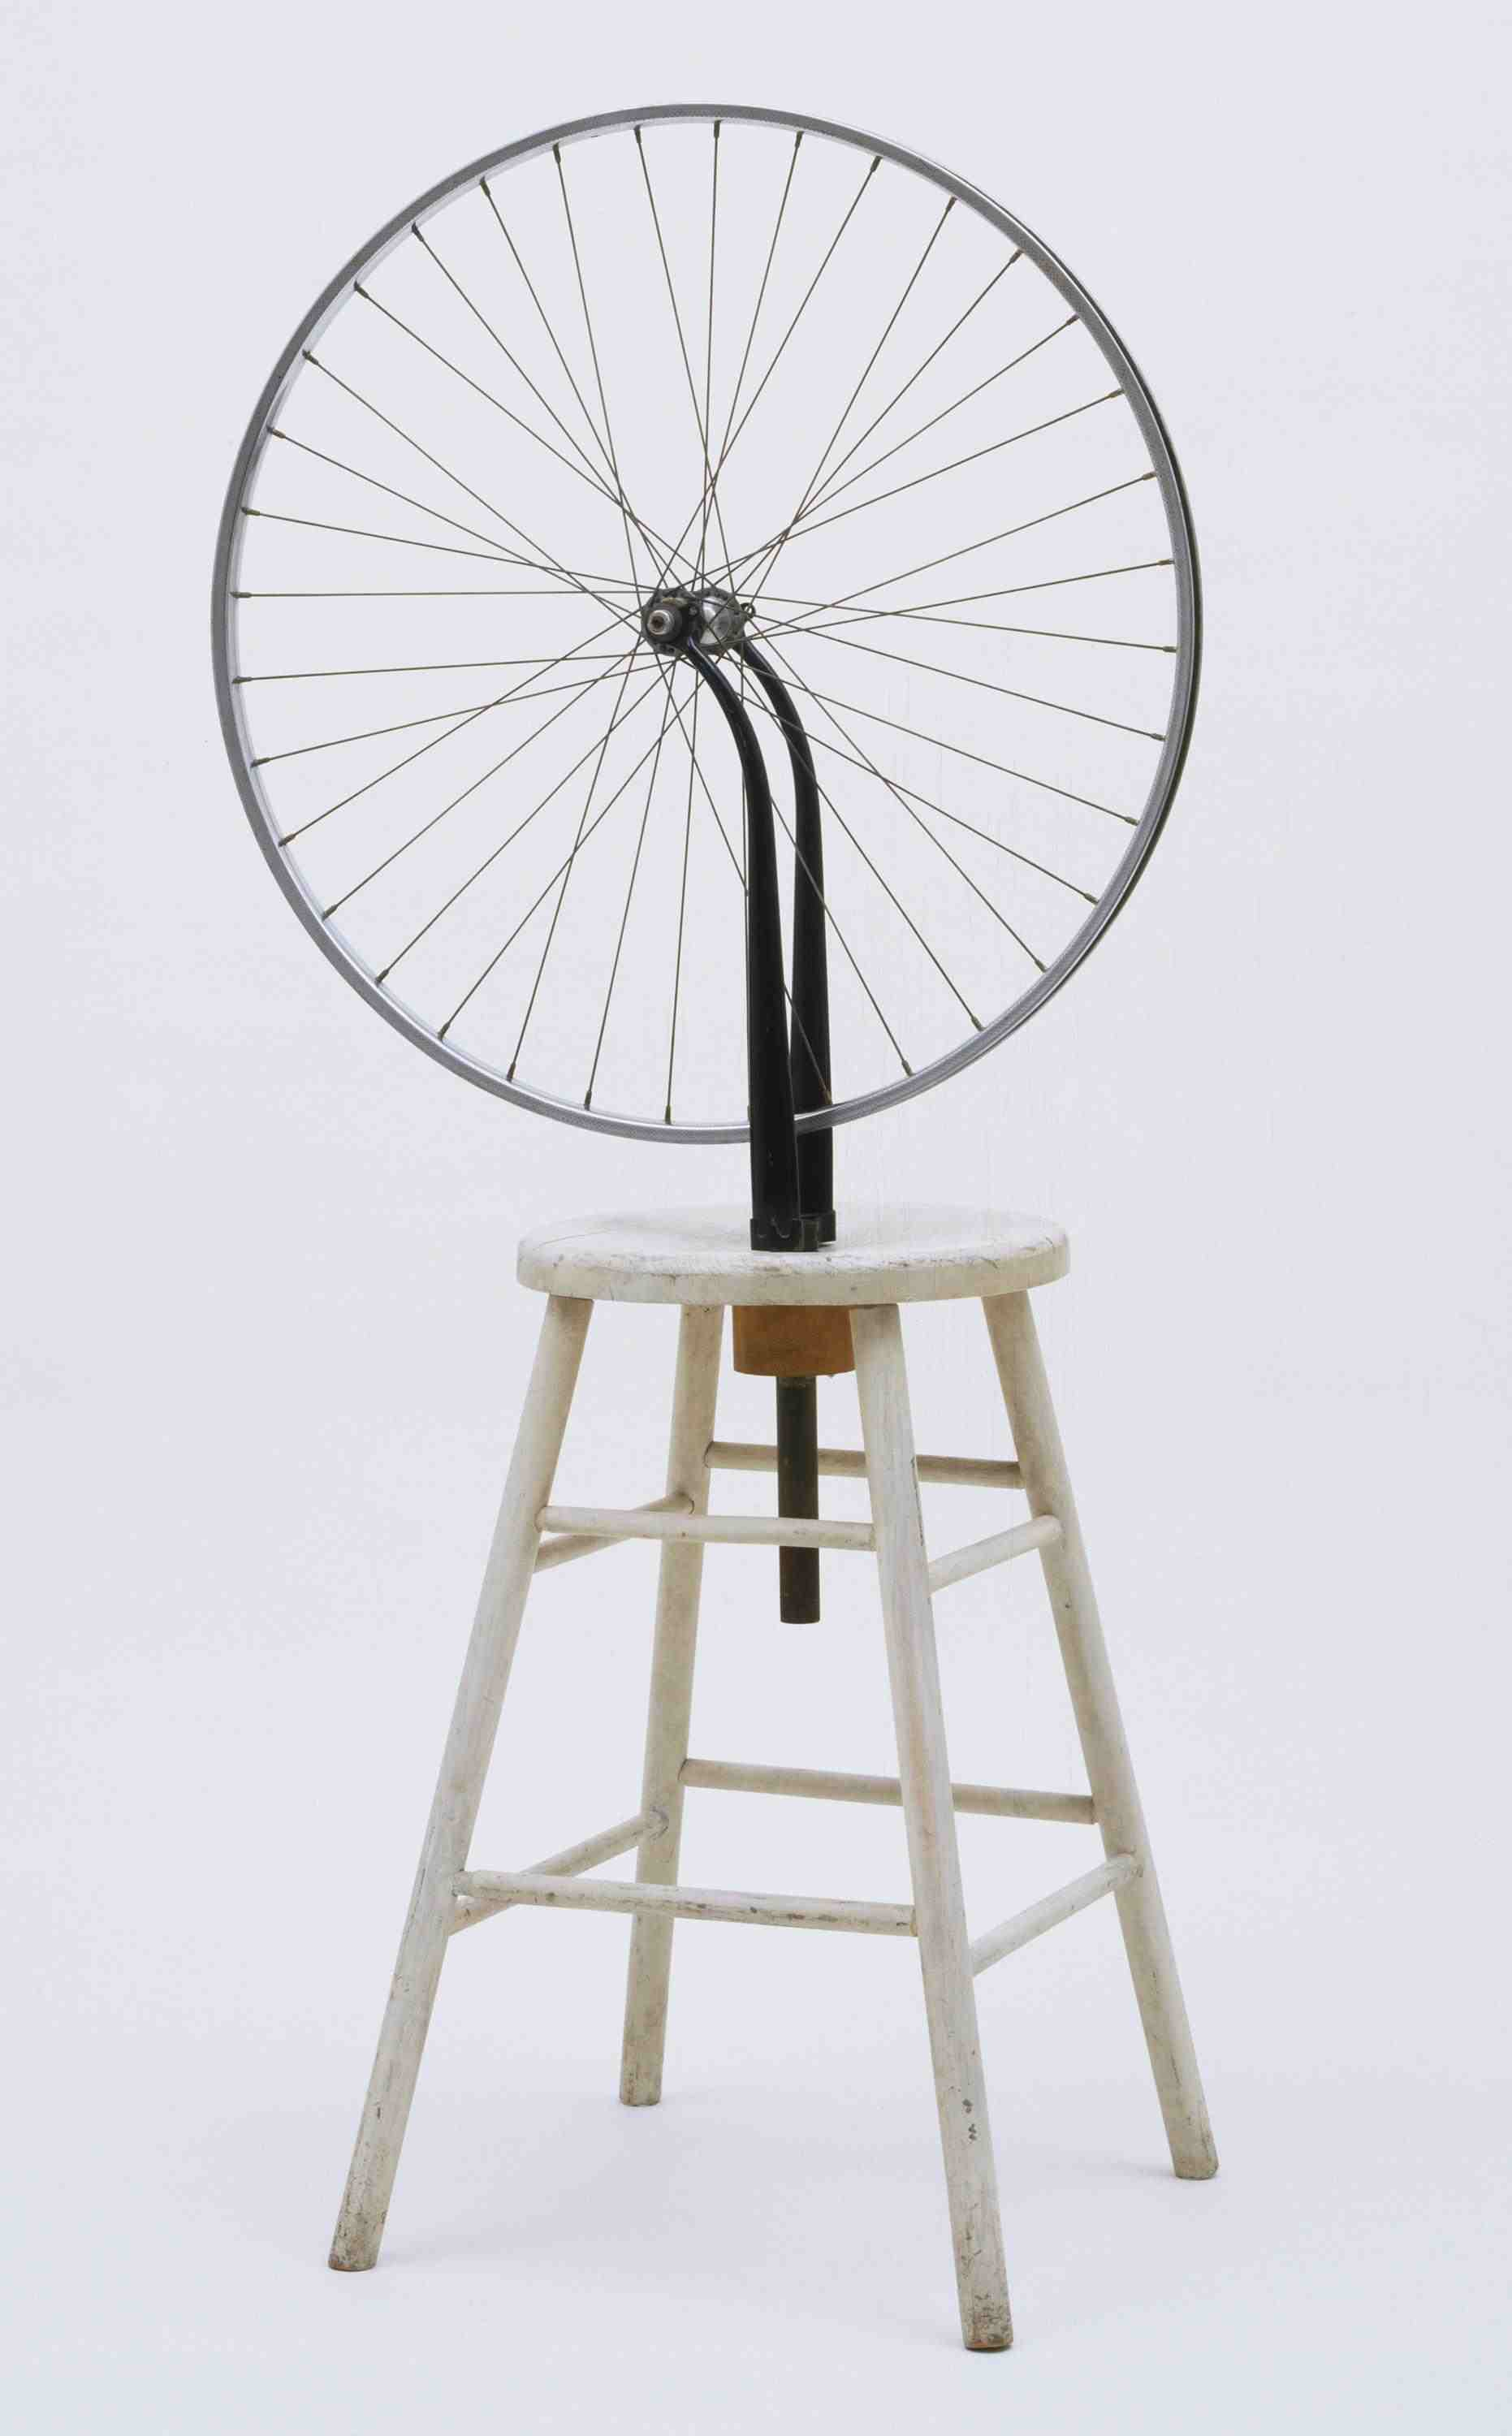
\includegraphics[height=6cm]{graphics/duchamp-bicycle-wheel-1913.jpg}
  \caption{Marcel Duchamp, Bicycle Wheel, 1913 (authorised reproduction 1951, original lost)}
  \label{fig:Duchamp_BicycleWheel}
\end{figure}





% TODO Bunu sadece referans olarak kullanabilirsin, çünkü zaten çok fazla tekrar var.
%\paraphrase{The use of trash as a fine art medium dates back at least to the work of early-20th-century artists such as Fortunato Depero and Kurt Schwitters. Use of found materials, including garbage, has been associated with assemblage art since the 1950s and has been practiced by other well-known artists, including graphic artist Christian Boltanski, sculptor Louise Bourgeois, and photographer Andres Serrano. Art made from garbage has since become much more common in fine arts venues such as museums, galleries, and high-profile installations, including H. A. Schuldt’s famous “Trash People,” which has traveled around the world since 1996 \cite{tauxe2012encyclopedia}.}

% TODO rubbish theoryinin başına konulabilir, referans olarak kullanılabilir.
% Book: Recycled, Re-Seen: Folk Art from the Global Scrap Heap
%\comment{Different meanings for everybody.} 
%\paraphrase{It is stated that same object can have one meaning for one community or culture and another meaning or series of meaning for another. Different objects have different life spans --- different degrees of permanence or disposability --- and that these life spans are socially constituted is also an integrated part of the story \ldots geographic and socioeconomic boundaries of class, caste and culture throughout the world. It is story of people --- the women, men, children etc. one person's trash into another's treasure.}

% TODO MOVE TO COMMON APPROACH
%\comment{Semiotic Context, juxtapositions} \paraphrase{"In popular writing (such as novels), in television, films, music, and other forms of mass expression, the term trash is used to signify work that is of especially low value." \cite{lukas2012garbage}}




%
%
\summary{Found Object} 
Found object originates from the French \textit{objet trouvé}, describing art created from undisguised, but often modified, objects or products that are not normally considered art, often because they already have a non-art function.

% TODO will not be used. just for rerefence
% Book: Recycled, Re-Seen: Folk Art from the Global Scrap Heap
%\comment{GIFT FROM GOD, NOT KNOWING PREVIOUS STATE} They also states that the practice of tribal people artfully transform Coca-Cola bottle (given as example by the authors). From western trash to tribal treasure. \paraphrase{For the Kalahari Bushmen, the process appears to be one not so much of reusing but of creating anew; not so much transforming, a inventing (p.9).} It stated these found objects is accepted as a gift from gods. A disposable item becomes imminent desire and profound social consequence. (Intercultural recycling.) \paraphrase{Both presentations tell a story about an aesthetic and cross-cultural process --- as well as an economic and political one --- which is defined by the act of recovering and transforming the detritus of the industrial age into handmade objects of renewed meaning, utility, devotion, and sometimes arresting beauty (p.10).}

% TODO will not be used. just for reference
% Book: Recycled, Re-Seen: Folk Art from the Global Scrap Heap
%[Having different meanings] For the same people are not used the items that are scavenged by people who have little or no contact with those who first possessed them, and may neither know nor care about their originally intended function. It is case from the film and also the case depicted in the real life photographs taken by anthropologist michael leahy which document his first colonial contact with new guinean highlanders.

% TODO will not be used. just for reference
% Book: Recycled, Re-Seen: Folk Art from the Global Scrap Heap
%\todo{yerlinin fotoğrafı}
%\quotes{Renowned early-twentieth century anthropologist Michael Leahy encountered a Wabag man from Papua New Guinea wearing an aluminum whole wheat biscuit tin on his head. In the symbol system of this culture, large, bright, and shiny ornaments are connote health, well-being, sexual attractiveness, and the approval of the ancestors.} \todo{ref.}





%(Summary From Paul M Camic.) 
%The term found object, as used in this article, refers to an existing object or artifact that is picked up (found) and generally not bought or originally intended as art, yet it is also considered to have some value (e.g., aesthetic, novelty, remembrance) to the finder. It is during the locating and finding process that the value of the object, once considered to be junk or rubbish, changes. The junk object becomes transformed into the valued found object. Objet trouve, translated from the French as “object found,” appears to have been first used by Marcel Duchamp in 1913 in reference to objects he made use of in his “readymade” art (Richter, 1965). His earliest known application for an objet trouve was seen in his well-known piece Bicycle Wheel, “where he had simply upturned a wheel on a stool” (Gale, 1997, p. 97) and labeled it a work of art. A more public and controversial introduction of the readymade occurred in 1917 when Duchamp attempted but failed to exhibit the highly contentious piece The Fountain, where a single white urinal became a readymade piece of art (Tomkins, 1996). These pieces were the beginning of Duchamp’s shift from an art striving for beauty and possessing a higher complex or hidden meaning beyond what was seen to an art form that made use of, and occasionally celebrated, the common materials and objects found in everyday living.

\paraphrase{Gascoygne (1936), writing about the artist’s use of “the strange medley of materials” (p. 169), referred to as objets trouve in Surrealist art, suggesting that the artist “discovers a hidden symbolic significance in the [found] object which is preserved when the object is ‘framed’ as art” (p. 170). The finder discovers an unrealised significance in the object. A new boundary is formed around the object by the finder through removing it from its found environment and placing it in a new one, thus empowering the finder in the role of creating a new reality for the object. He argued that the found object, before it is found, approximates a zero value aesthetically; the zero value increases for the finder---beholder on discovery of the object and increases further if the object is placed in another context. \ldots the meaning of material objects was derived from their symbolic relation to another (e.g., person, time, place, experience) rather than through their physical attributes (Causey, 2003; Csikszentmihalyi \& Rochberg-Halton, 1981).} \todo{parap. ref.}

\paraphrase{Artifact exploration promotes historical thinking, literacy investigation, and cultural expression (Higgs \& McNeal, 2006; Levstik \& Barton, 2001; Morris, 1998). Meanings are embedded within cultural artifacts and language (Vygotsky, 1978).}

%How a region of flexibility develops, what social factors are involved in taking innovative and creative responses toward rubbish, and how an individual changes (and enhances) his or her creative responses toward society’s detritus are areas that require additional examination. (Important points a gap in the literature. Although Parsons article analyze practices, it is not very broad and detailed. Further what is the importance of it is missing.)

%The importance and enjoyment of found objects to those who participated in this study, using them in various ways and for different reasons, were strongly evident. The interaction between finder and object is an attempt to make meaning of an object that has been found, and by being found and desired becomes transformed.

%Gascoygne (1936) recognized that finding an unrealized significance in a material (found) object was empowering partially because, through the creative agency of the finder, the object’s aesthetic value had increased from zero to something greater. The transformation of rubbish from a negative value to a positive value requires the finder to develop a symbolic meaning, and sometimes a functional use, for the object that goes beyond its present situation as culturally labeled detritus while simultaneously responding to its current physical and aesthetic elements. When the found object is seen by the finder as a symbol representing another entity (e.g., when an old blue bottle with foreign lettering comes to symbolize far away intrigue, mystery, and sophistication), support is given to what Dittmar (1992) described as socially constructing a material identity for the object. Expanding on Dittmar’s use of a social interactionist perspective, the results of the present study support the possibility that the entire found object process---finding, reclassifying, and reusing objects---becomes a symbol of identity for the finder. This supports Digby’s (2006) argument that individuals make use of salvaged objects as souvenirs, which are no longer part of the commodity cycle, to rework and construct individual and social identities.

%An important difference, however, which also appears to contribute to the aesthetic experience, takes place when discovering an object unexpectedly in a nonpredetermined place and time. Unlike appreciating art in a museum, which is a boundaried activity occurring at a scheduled time and place with the anticipation of finding and looking at art objects, finding discarded objects can occur anywhere at anytime and thus, according to participants, can “trigger” a burst of sensory attention and a “surge” of cognitive activity on the part of the finder. 

%Results of this study also support consideration of found objects as important artifacts that are signifier of cultural meaning.

% [TODO adapt for my case] Found objects first came to the attention of the general public through their use by artists in early part of the 20th century. To help contextualize the application of found objects, the following section provides an overview of their use by Western artists. This is followed by an examination of objects in human development and includes aspects of psychoanalytic theory, material objects and their relationship to identity, selected cognitive theories, and an outline of the social life of objects through rubbish theory.





%
%
\section{Examples from contemporary artists}
In the light of discussions at previous section, some of the works (or current strategies and approaches ) of artist are analyzed. First one is related with found objects.

% Neden bu işler, neden bu sıra?

% Neden çöpü kullanıyorlar. Bunu belirmek gerekli. İlki sanata farklı bir obje sokarak saflığını bozma, hazır yapım ile geleneksel yöntemlere karşı çıkış, fikrin ön plana çıkması. Visual uniqueness, aesthetics dimension, Economic reasons

Photobooths are machines that place crowded places and with affordable cost people can get their photos. It is a pheonema that attract attention of artist and researchers such as Martin Parr and Gerry Badger who published history of them as a two volume.

In the French film Amélie\footnote{Original title: Le fabuleux destin d'Amélie Poulain, in english: The Fabulous Destiny of Amélie Poulain} directed by Jean-Pierre Jeunet in 2001, young male character collects photos that are torn up and thrown away by their owner near photo booths spread through train and metro stations of Paris. He collects them and glue them together in a photo album. In the film photo booths and found photos are central catalytic. Amélie falls in love with him when she realize him searching for found photos. After his photo album passed to Amélie, she looks every page of photo album again and again. Through the images of unknown people, she establishes narratives that point out the significance of these images even if they are thrown away. The important part of the film it generates images of a man who scanvage the photos of another people. There are a lot of artist who collects discarded items but their process is not well documented. Therefore we are not aware of the artist process. 

\begin{figure}[h!]
  \centering
  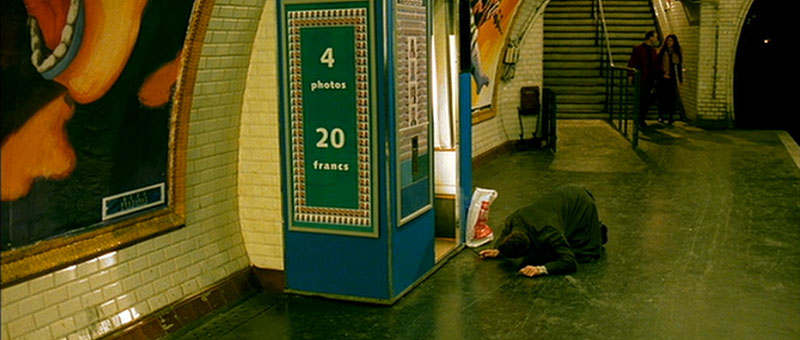
\includegraphics[height=6cm]{graphics/amelie_01.jpg}
  \caption{Still image from Amélie}
  \label{fig:Amelie}
\end{figure}

Prior to film Amélie, British artist Dick Jewell published a book in title of "Found Photos" in 1977. It is a collection of photobooth images that had been thrown away or torn up by the people in the photos. Ian Walker comments on that it is "always a joy to look through." Images capture diverse range of activities and expressions of people using photo booth machine. They are scavenged by the artist from the photo booths of London. The reasons of why photos are rejected vary including technical problems like flash or posing time. On the other hand, some of them are very good condition, and it is a mystery that why they are rejected. Walker explains that the \todo{block qoute} "gap between our exterior perception of the image and what must have been the internal dissatisfaction of the original subject results in some of the effective moments in Found Photos, where the images are not only bizarre and wonderfully funny (as many of them are) but also profoundly moving." Walker argues that even if photo booths are mechanic and simple application of photography while capturing everyday life, leave behind such ambiguous and mysteries that some people trace them. "Dick Jewell’s approach with Found Photos was less interventionist, presenting the images themselves in the spirit of either an anthropologist showing his finds or a conceptual artist claiming bits of the real world as ‘readymades’." His mode of discovery includes climbing to look at the top of the box and looking for the nearest waste bin. Badger describes Found Photos as ‘both a conceptual artwork and a sociological footnote’.

\begin{figure}[h!]
  \centering
  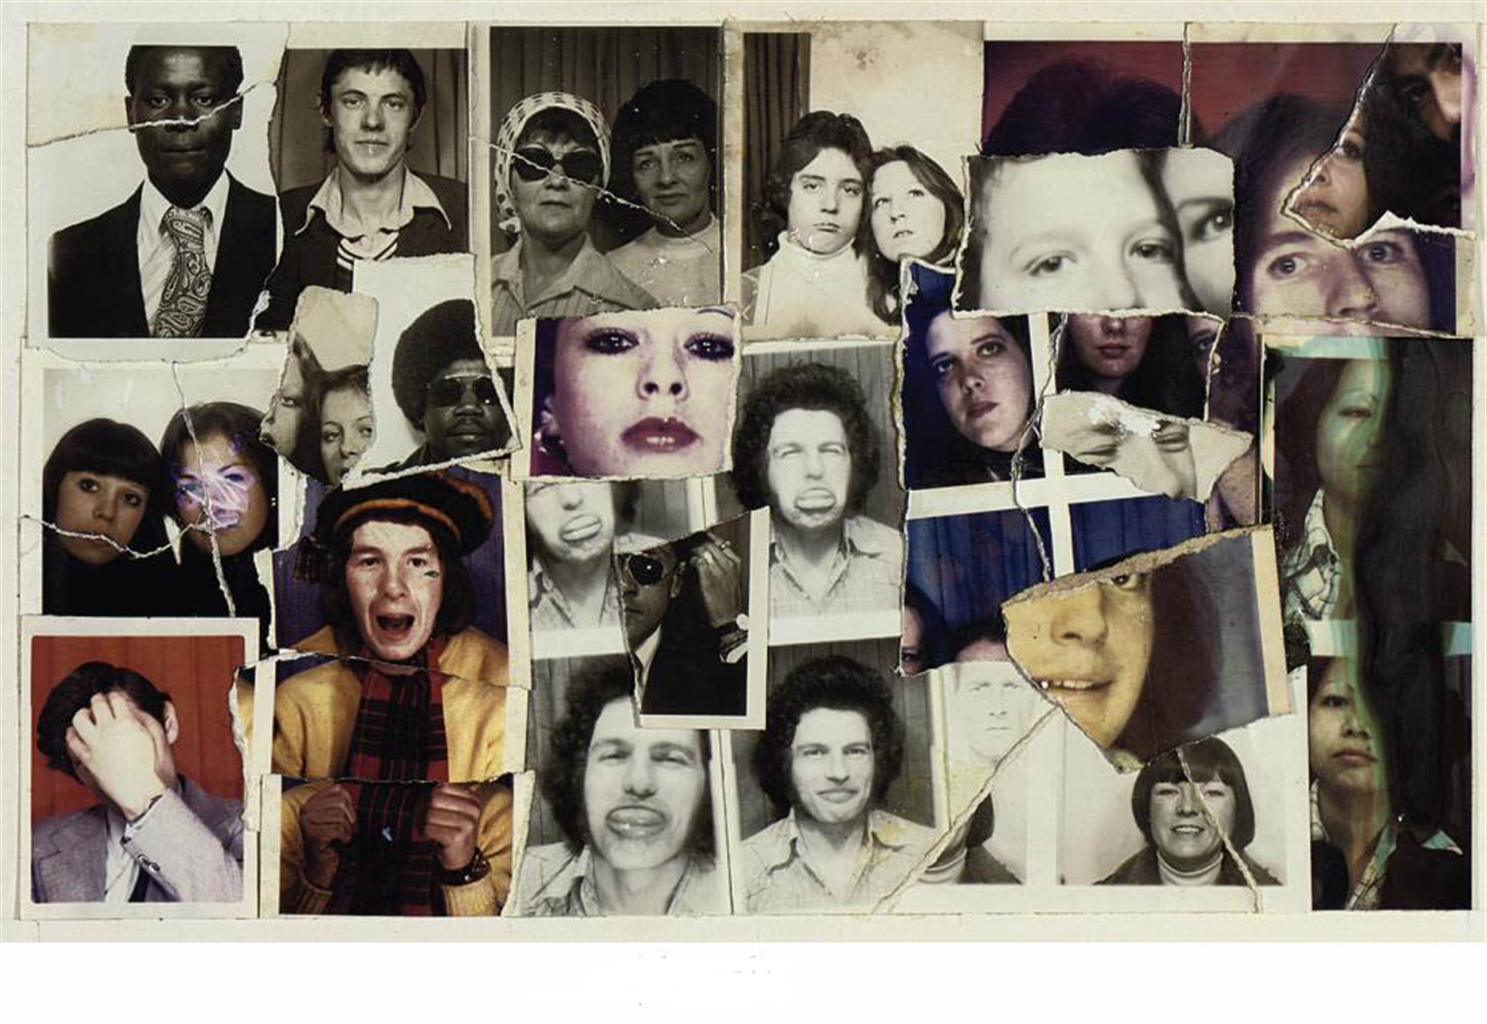
\includegraphics[height=6cm]{graphics/DickJewell_FoundPhotos.jpg}
  \caption{Dick Jewell}
  \label{fig:DickJewell_FoundPhotos}
\end{figure}

On the other side for another artist photographs serve a function to record his daily trash. Tim Gaudreau photographed every object that he threw away for one year. At the end around five thousand images are covered all the gallery and opened to visitors. He notes that it just started as a documentation of his discards, but later it became (part of his life and) an obsession that he can not able to easily quit off. He says that "this collection of images intimately displays what I do, what I consume. It reveals me." Like in the case of Tracey Emin trash turns to a medium that is used to express oneself. People are not only composed of the listed items in the CVs like in the film Fight Club Tyler Durden draws attention to the narrator by saying: "You are not your bank account". It is an effective way of looking things left behind rather that things put forward. Through this project, artist reached better understanding what he is and notes that this project changed his consumption choices and patterns.

\begin{figure}[h!]
  \centering
  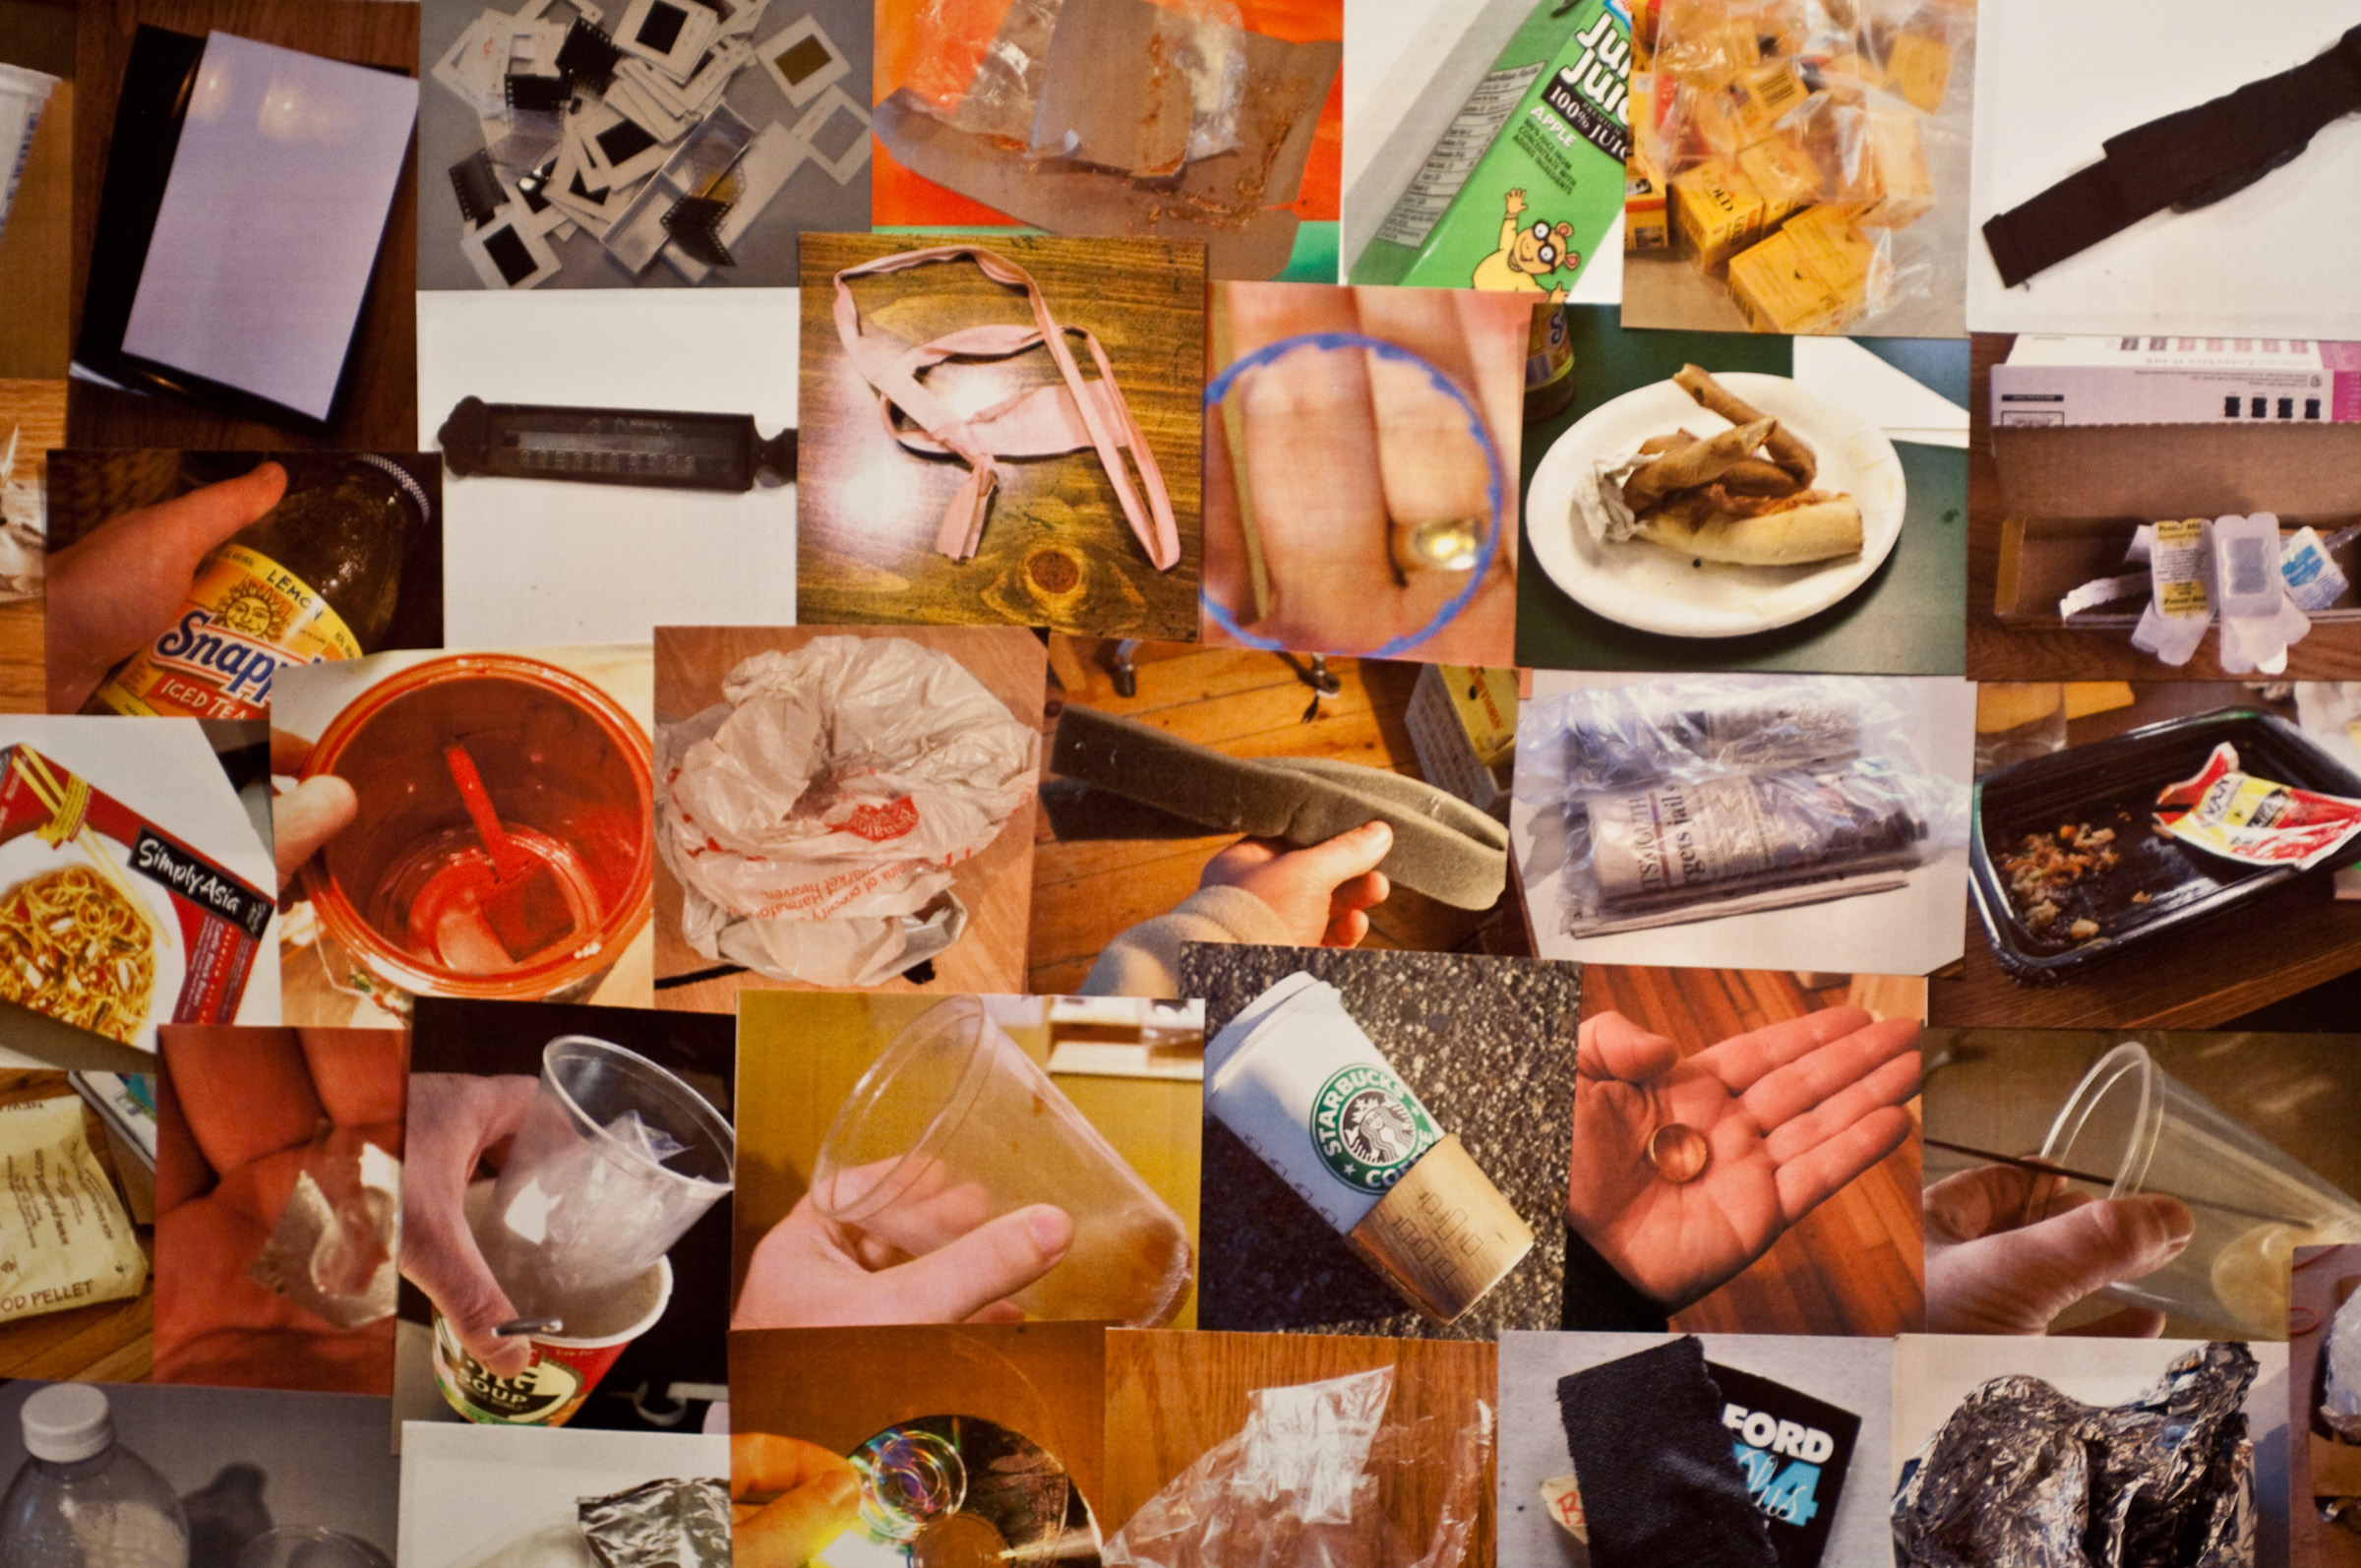
\includegraphics[height=6cm]{graphics/TimGaudreau_SelfPotraitRevealedByTrash.jpg}
  \caption{Tim Gaudreau, Self-Portrait as Revealed by Trash: 365 days of photographing everything I threw out – Variation I, 2006}
  \label{fig:TimGaudreau_SelfPotraitRevealedByTrash}
\end{figure}

Filomena Cruz turns her lens to the city and its trashes that are left behind, thrown away and squeezed on the sidewalk or pavement. In her photographic series "Road Kill", she captures tiny "trash corpses" that are generally ignored and out of sight. In other words, the skin of city revealed through her photos in micro scale. On the skin of city there are lots of trash including "a piece of chewing gum with an "engraved" leaf; a flattened-out tube; a corroding paper napkin with a still intact heart; or a frog-green Crayola melting in the heat, all speak the language of "worthlessness" suddenly becoming meaningful" as looked through the window of they capture the city life and skin of the city that we touched. She shows us tiny details of huge cities. (Somehow these trashes for all effort succeeded to stay in the towns.) These trashes can not be removed from the city but moved ones are stacked on landfill, and they are not tiny as they are.

\begin{figure}[h!]
  \centering
  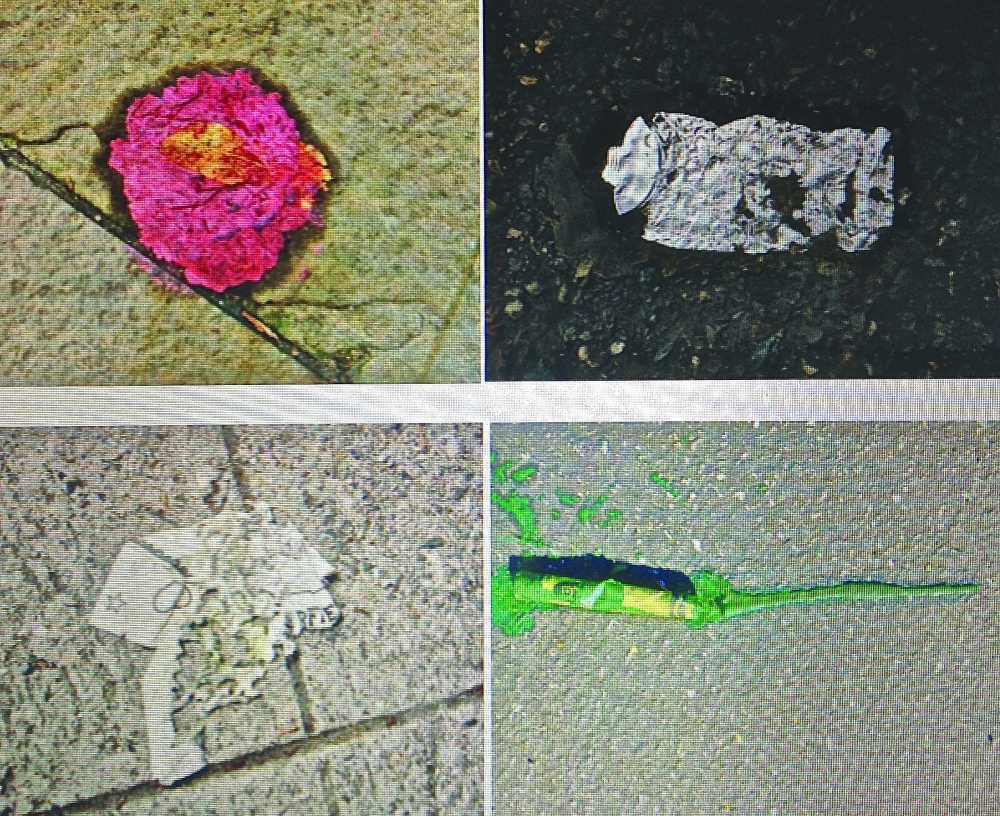
\includegraphics[height=6cm]{graphics/FilomenaCruz_RoadKill_ReVista.jpg}
  \caption{Road Kill by Filomena Cruz}
  \label{fig:FilomenaCruz_RoadKill_ReVista}
\end{figure}

In the documentary film, Waste Land, Vik Muniz frames portraits of \textit{catadores} who are pickers of recyclable materials on the dump. He visits them at one of the biggest open-air garbage dump outside of the Rio de Janeiro home of the millons of people. Film documents whole process of development and production of "Pictures of Garbage" made of collected trash from dump. He selects unusual materials and people for potraits rather than the powerful and notable people as commonly encountered at Renaissance. To create portraits of \textit{catadores} there is any other material than trash because of they are already build up their life in trash of city. [Also these image are sold an auction and earned money donated to the \textit{catadores}. The images of trash moved to beloved places such as homes and museums. As stated in the rubbish theory they transformed to a durable object.]

\begin{wrapfigure}{r}{0.4\textwidth}
  \begin{center}
    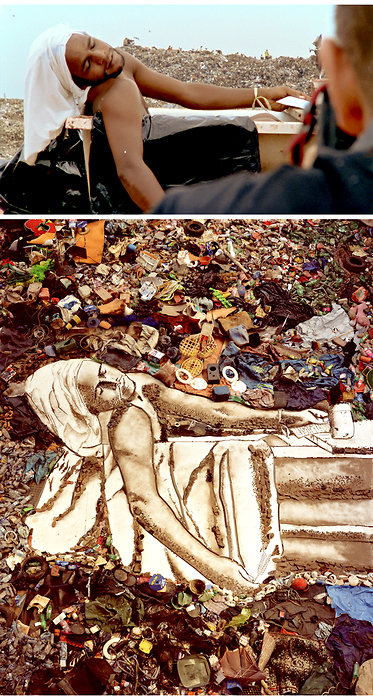
\includegraphics[width=0.37\textwidth]{graphics/vik-muniz-picturesofgarbage0.jpg}
  \end{center}
  \caption{Vic Muniz, Pictures of Garbage}
  \label{fig:VicMuniz_PicturesOfGarbage}
\end{wrapfigure}

Not only monumental portraits extracted from the dump but also an orchestra is grounded up from the dump of Paraguay pioneered by Favio Chávez and Nicolás Gómez. Favio Chávez is a music teacher, and Nicolás Gómez is a garbage picker. They live in Cateura at Paraguay. It is a one of the poorest villages where people live among the sea of garbage. "A violin is worth more than a house here," says Favio Chavez in documentary film. The orchestra's director and founder. Favio Chavez director and founder of the orchestra whose instruments such as violins, flutes and cellos are built from collected trash by Nicolás Gómez. Players of the orchestra are compiled from the children who are hopeless for their future. In the midst of such an existence, these musicians have created something both special and truly awe-inspiring. They are given birth to an orchestra that plays the masterpieces of classical music composed by Mozart, Beethoven, and Vivaldi. Trash turned to treasure and totally ironic that a signifiers of high culture like classical music can be even played with imperfect instruments. For them and also, most of the people it is not affordable to buy an instrument and get the education of classical music. (To enjoy and play such music requires economic wealth and it is not possible for everyone.) What they create is actually not expected from them, and their success is not limited with their location. They have given concerts around the world. 

%"People realize that we shouldn't throw away trash carelessly," says Chavez at the end of the trailer. "Well, we shouldn't throw away people either." \quotes{The world send us garbage. We send back music}.

% Resistance to all hard conditions

\begin{figure}
    \centering
    \begin{subfigure}[b]{0.47\textwidth}
        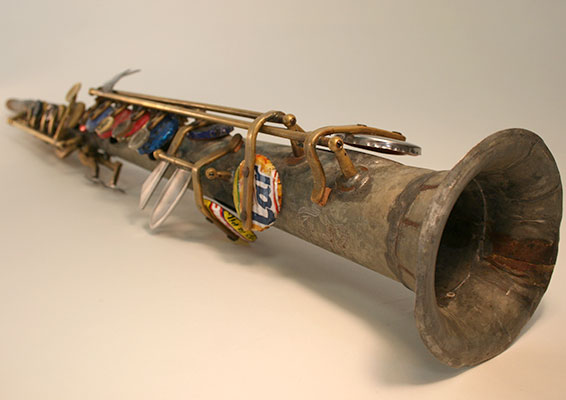
\includegraphics[width=\textwidth]{graphics/landfill_harmonic-sax.jpg}
        \caption{Sax}
        \label{fig:landfill_harmonic-sax}
    \end{subfigure}
    \begin{subfigure}[b]{0.47\textwidth}
        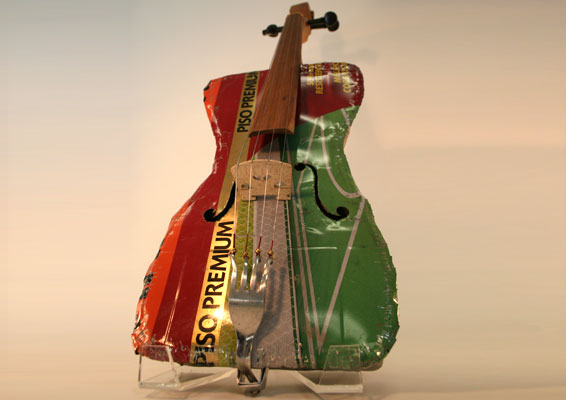
\includegraphics[width=\textwidth]{graphics/landfill_harmonic-violin.jpg}
        \caption{Violin}
        \label{fig:landfill_harmonic-violin}
    \end{subfigure}
    \caption{Instruments of Recycled Orchestra}\label{fig:animals}
\end{figure}

As noted that recycling as an economic strategy of survival in developing countries throughout the world. Creative production that is motivated, primarily, by adverse conditions of economic necessity. Economic survival and adaptation are influential factors for both the makers, who build an informal business on the making and selling of recycled goods and the local consumers, for whom the market for affordable, utilitarian goods is devised. (p25)

They build their musical instruments from what is available around. This project can be seen as a bricolage practice. Dictionary meaning\todo{which dictionary}; something constructed using whatever was available at the time. \paraphrase{Claude Levi-Strauss notes that the \textit{bricoleur} works not from the principle of making things only if natural resources are available but makes things according to those things at hand, making do with what is available. It is an expression that, like the natural cycles of the Earth, attempts to make something new from something old. \cite{levi1966savage}} The \textit{bricoleur} is \ldots someone who works with his [or her] hands and uses devious means compared to those of a craftsman \ldots \cite{levi1966savage} 

\paraphrase{\ldots someone that creates bricolage is described as a bricoleur, an odd-job man who works with his hands, employing the bricoles, the scraps or odds and ends.}

\begin{quote}
[He or she] is adept at performing a large number of diverse tasks; but, unlike the engineer, he [or she] does not subordinate each of them to the availability of raw materials and tools conceived and procured for the purpose of the project. His [or her] universe of instruments is closed and the rules of his [or her] game are always to make do with “whatever is at hand,” that is to say with a set of tools and materials which is always finite and is also heterogeneous because what it contains bears no relation to the current project, or indeed to any particular project, but is the contingent result of all the occasions there have been to renew or enrich the stock or to maintain it with the remains of previous constructions or destructions.\cite{levi1966savage}
\end{quote}

%\begin{quote}
%The bricoleur, says Levi-Strauss, is someone who uses 'the means at hand,' that is, the instruments he finds at his disposition around him, those which are already there, which had not been especially conceived with an eye to the operation for which they are to be used and to which one tries by trial and error to adapt them, not hesitating to change them whenever it appears necessary, or to try several of them at once, even if their form and their origin are heterogenous---and so forth. There is therefore a critique of language in the form of bricolage, and it has even been said that bricolage is critical language itself\ldots If one calls bricolage the necessity of borrowing one's concepts from the text of a heritage which is more or less coherent or ruined, it must be said that every discourse is bricoleur.\cite{derrida1993structure}
%\end{quote}

%\begin{quote}
%The engineer, whom Lévi-Strauss opposes to the bricoleur, should be the one to construct the totality of his language, syntax, and lexicon. In this sense the engineer is a myth. A subject who would supposedly be the absolute origin of his own discourse and would supposedly construct it 'out of nothing,' 'out of whole cloth,' would be the center of the verbe, the verbe itself. The notion of the engineer who had supposedly broken with all forms of bricolage is therefore a theological idea; and since Lévi-Strauss tells us elsewhere that bricolage is mythopoetic, the odds are that the engineer is a myth produced by the bricoleur.\cite{derrida1993structure}
%\end{quote}

% TODO Bunu bitirirken de bir şeyler demek gerekli.

In the scope of painting different than the works in the previous chapter (paintings on tea bags and coffee cups) historical potraits of notable people are painted onto the flattened aluminum drink cans which are disposable objects. The people in the figure X is General Jefferson C. Davis who was an officer at United States Army in 19th-century. Selected persons can be viewed as a member of the higher or ruling class of society. Therefore Kim Alsbrooks, painter of these works, might thought that to make trash is more valuable, their face will be good. Or the vice versa. She may use trash to provocate social elite of that time. 

\begin{wrapfigure}{r}{0.4\textwidth}
  \begin{center}
    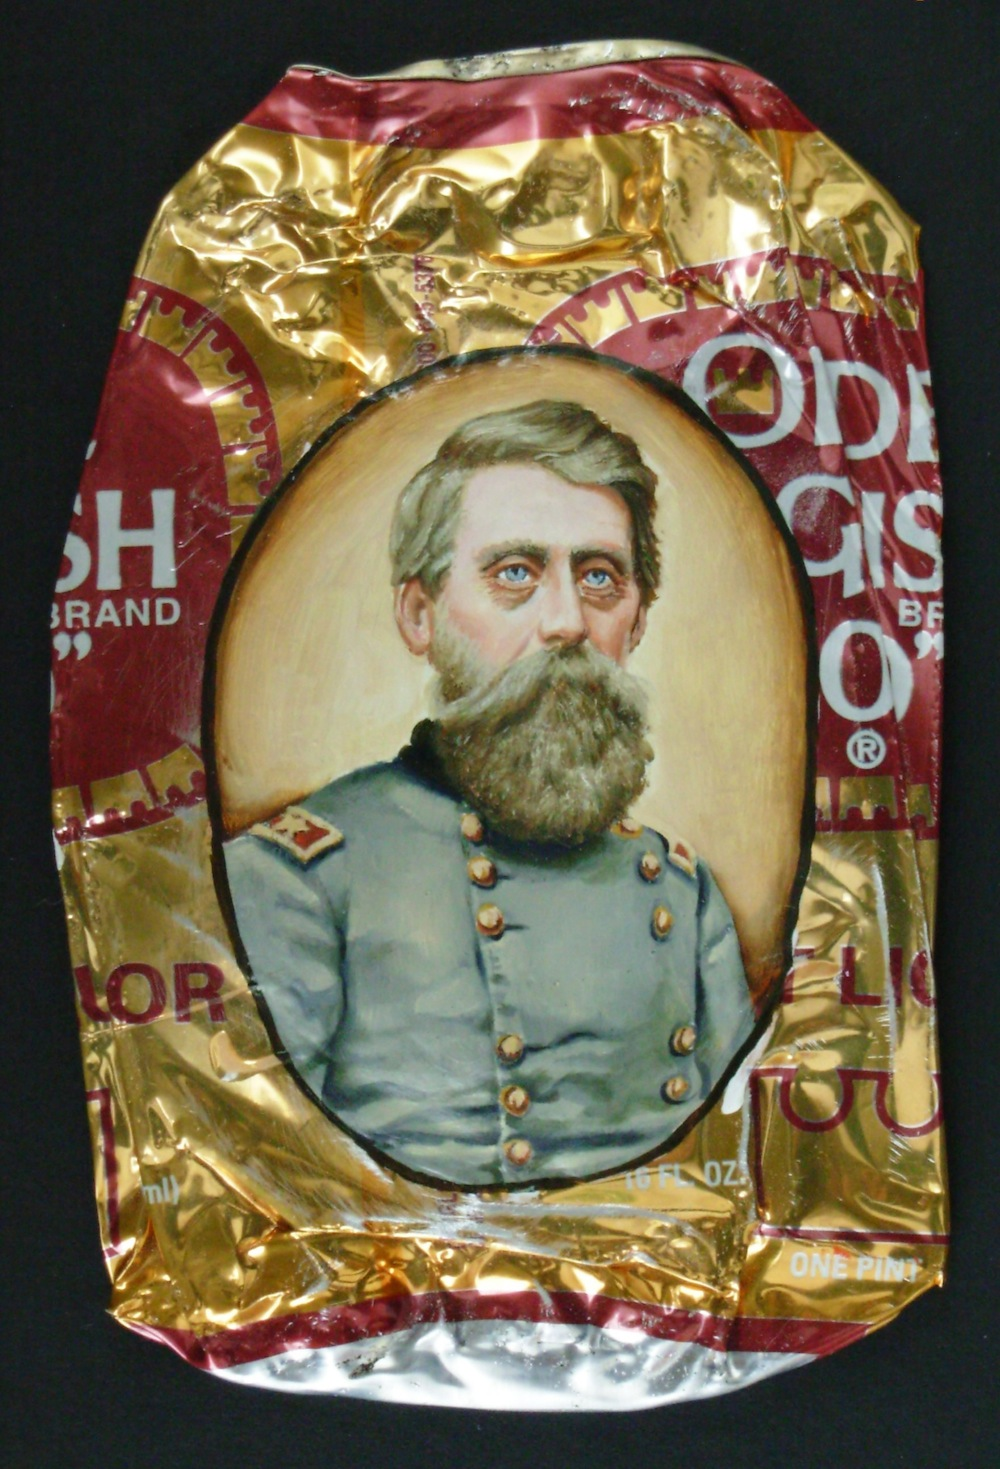
\includegraphics[width=0.37\textwidth]{graphics/Alsbrooks.jpg}
  \end{center}
  \caption{Kim Alsbrooks, The White Trash Series}
  \label{fig:Alsbrooks}
\end{wrapfigure}

Not all the time and every artist turn trash into different objects sometimes they trash them. Michael Landy's Art Bin is one of them. It is a room size transparent bin placed inside of the art gallery. He invites people to bring their own artworks of failed attempts. Some of the notable contemporary artists such as Damien Hirst, Gillian Wearing, Tracey Emin and Mark Titchner participated in by throwing their sculptures, paintings, and prints into the Art Bin. People publicly toss their work from a high platform, and all of them can be seen outside of the transparent walls. He listens to the story and the failure of the artworks from their creator, and it is not allowed to throw others work. At one side he criticizes the idea of not aware of that artist also have lots of failures. People only can see the final work in the galleries and museums. In this work he break-ups this notion that encouraging the artist reveals their failures to the public. Like his words, it is “a monument to creative failure”. (According to this approach one can extract that failures belong to the trash bin. However, there must be other alternatives that to demystify the practice of the artist.) On the other side, there is a provocative approach to the art and art objects by saying that "Nothing is too good for the art bin." There is no limitation of throwing away even if art. 

\begin{figure}[h!]
  \centering
  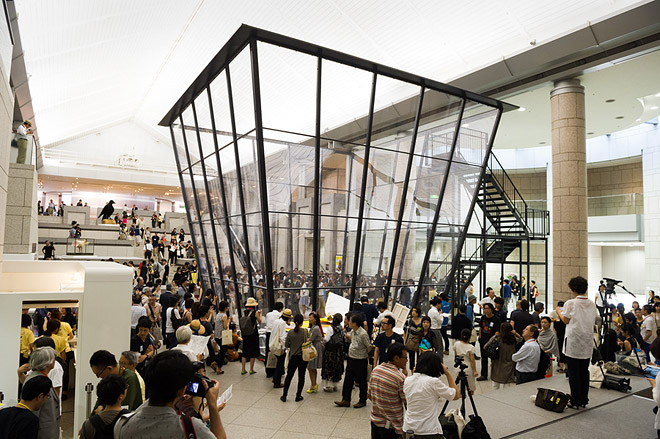
\includegraphics[height=7cm]{graphics/MichaelLandy_ArtBin.jpg}
  \caption{Michael Landy, Art Bin}
  \label{fig:MichaelLandy_ArtBin}
\end{figure}

Not all artist transform trash although some deconstruct them. Michael Landy is one of them. Michael Landy's Break Down Inventory is a two-week show (display) of destruction process of his all possessions on a dissemble line with the help of 10 workers. Firstly they are classified and recorded for three years and the deconstructed in two weeks by separating every element to the smallest part. Reveal all his possessions and deconstruct of them while he is alive. He turns them to rubbish and makes them unusable. Breaking down the all the meaning. Breaking down the connections. It can be an example of a downcycling process. It is preferred to decompose all the complex link and relationships between the objects. They are not just ordinary things they are possessions of the artist. Break Down 2001, in which he systematically destroyed all his personal possessions. His work examines what we value and what we discard, consumerism and waste, and human labor and its worth. It happens in public space. People can see the process. This process lasts two weeks at a place where people buy goods.

\begin{figure}[h!]
  \centering
  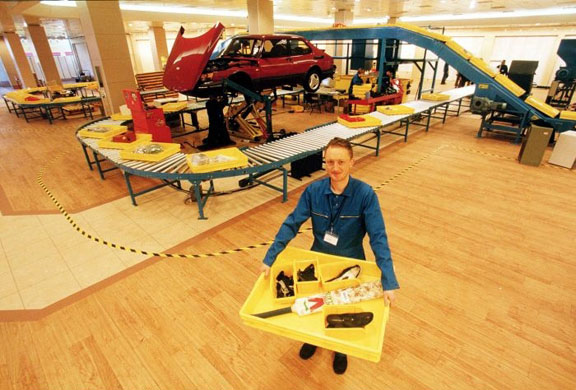
\includegraphics[height=7cm]{graphics/MichaelLandy_BreakDown.jpg}
  \caption{Michael Landy, Break Down}
  \label{fig:MichaelLandy_BreakDown}
\end{figure}

% TODO kendi işime taşıyacağım.
% http://www.publicbooks.org/interviews/recycling-literary-culture-a-conversation-with-lucia-rosa, http://www.eloisacartonera.com.ar/ENGversion.html
%\textbf{Eloísa Cartonera.} a work cooperative in Buenos Aires, proudly produces handmade books with cardboard covers. \quotes{We purchase [\ldots] cardboard from the urban pickers (cartoneros) who pick it from the streets. Our books are on Latin American literature, the most beautiful we had a chance to read in our lives.} \quotes{Some of them are preserved as art books at university libraries, while others circulate as literary pieces expected to disintegrate in time---something anticipated of the material they are made from.} [from PAOLA IBARRA, ReVista]

%It reminds me that litreary is also a combination of reused thing. Because to create meanings we reuse words and idioms again and again with different combination.

%\begin{figure}[ht]
%  \centering
%  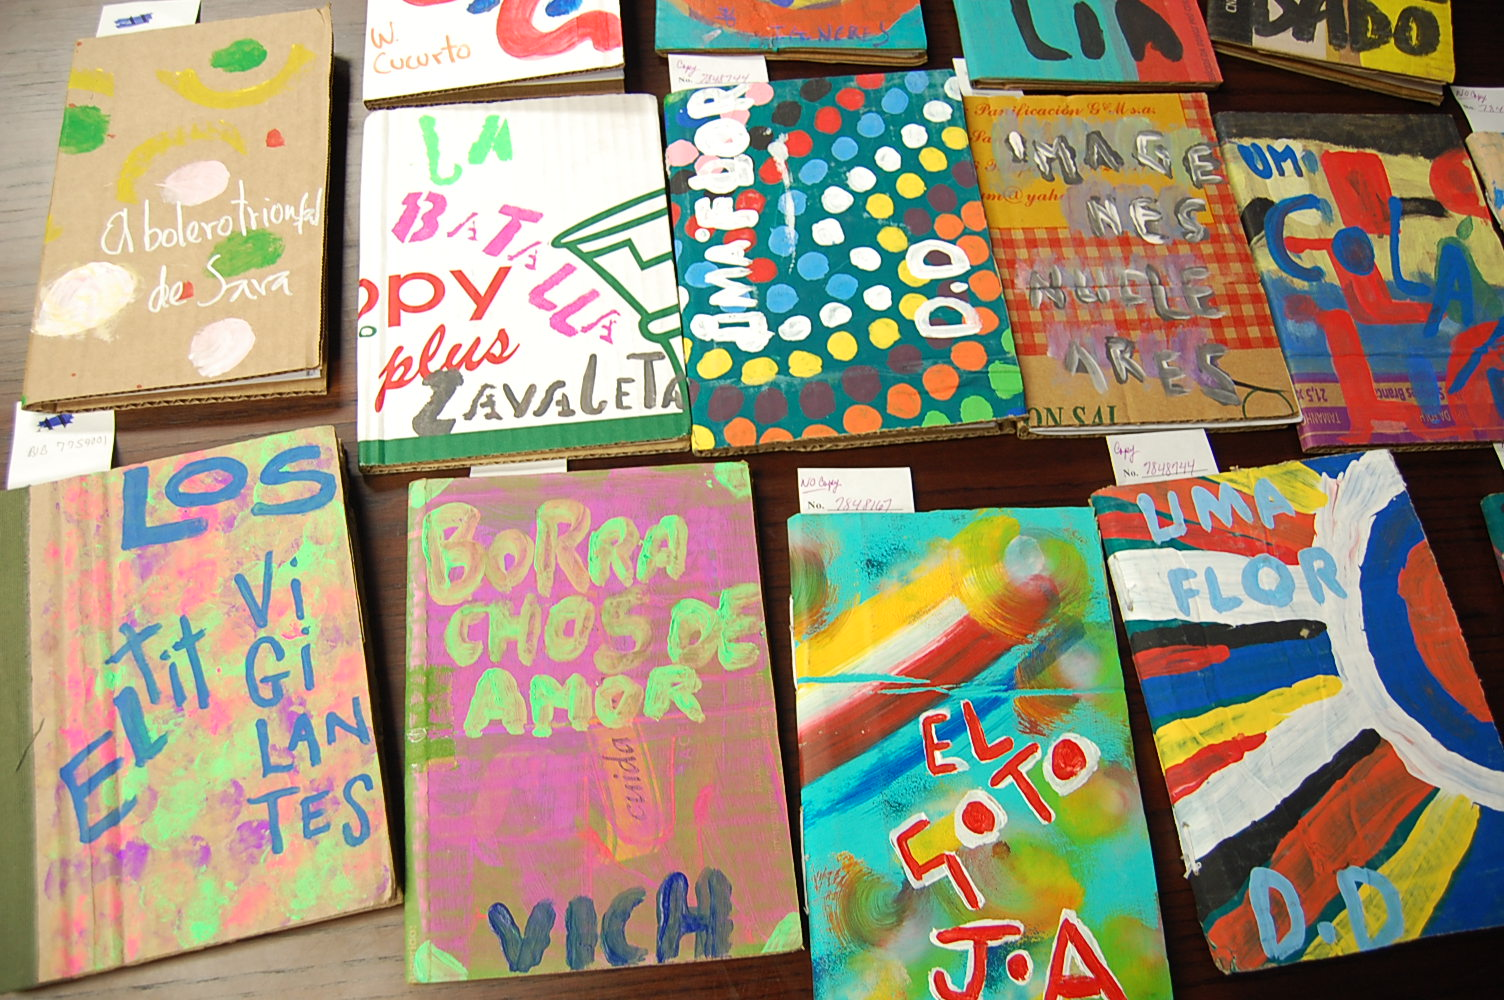
\includegraphics[height=6cm]{graphics/EloisaCartonera_Books2.jpg}
%  \caption{Books covered by Eloisa Cartonera}
%  \label{fig:EloisaCartonera_Books}
%\end{figure}

The film American Beauty, which features a long, poetic clip of a plastic bag swirling on an eddy of air yet people find it hard to think of plastic bags as things of beauty. But as a product -- as something created and then unleashed to become seamlessly integrated into the lives of millions of people around the world -- there is a strange allure to them, just as a pathologist can admire the structure of a particularly virulent and contagious virus.

Examples are not limited with these. Even if \paraphrase{trash is dirty and smelly trash can provide the raw materials for exquisite art---from sculpture to film and beyond.}





%
%
\section{The case of \quotes{The Gleaners and I}}
"The Gleaners and I" is a French documentary film directed by Agnès Varda in 2000. The film features various kinds of gleaning. According to the Merriam-Webster dictionary gleaning refers "to gather grain or other produce left by reapers". Varda searches for the historical and current practices of gleaning in rural and urban areas of France. Historically, gleaning is the act of collecting what is left and not profitable crops after the harvest. By combining different fragments through his film, she shows that the act of gleaning also exists in various forms and styles. In particularly she curiously focuses on the (un)familiar people who glean leftover of society. Moreover, it is a self-reflexive film because the director establishes a relationship with the practice of gleaners and her filmmaking practice. Some people glean crops; the others discarded food, and Varda gleans images.

The film is more than a research and document of the lives of many gleaners. It highlights the degree of global consumerism of the modern world and how technological advancements (or industrial (technical, modern) standards) result in waste. Varda seeks the several stages of potatoes from producers to consumers. As she discovers that supermarkets, buy only potatoes that fit in industrial standards of shape and size. So what happens to the others? Varda discovers and shares with us the disturbing fact that they are taken back to the field where they came from, by following with the camera the trucks that unload mountains of potatoes. As Rosello notes that "The ‘good’ potato is not the edible potato but one that will fit into a plastic container to be displayed on the shelf of a supermarket." Varda records few people who glean the rejected potatoes from the field, and also she joins them by collecting heart shaped potatoes that fascinate her. Rosello explains that she is collecting not only refused potatoes but also images that are left behind.

\begin{figure}[h!]
  \centering
  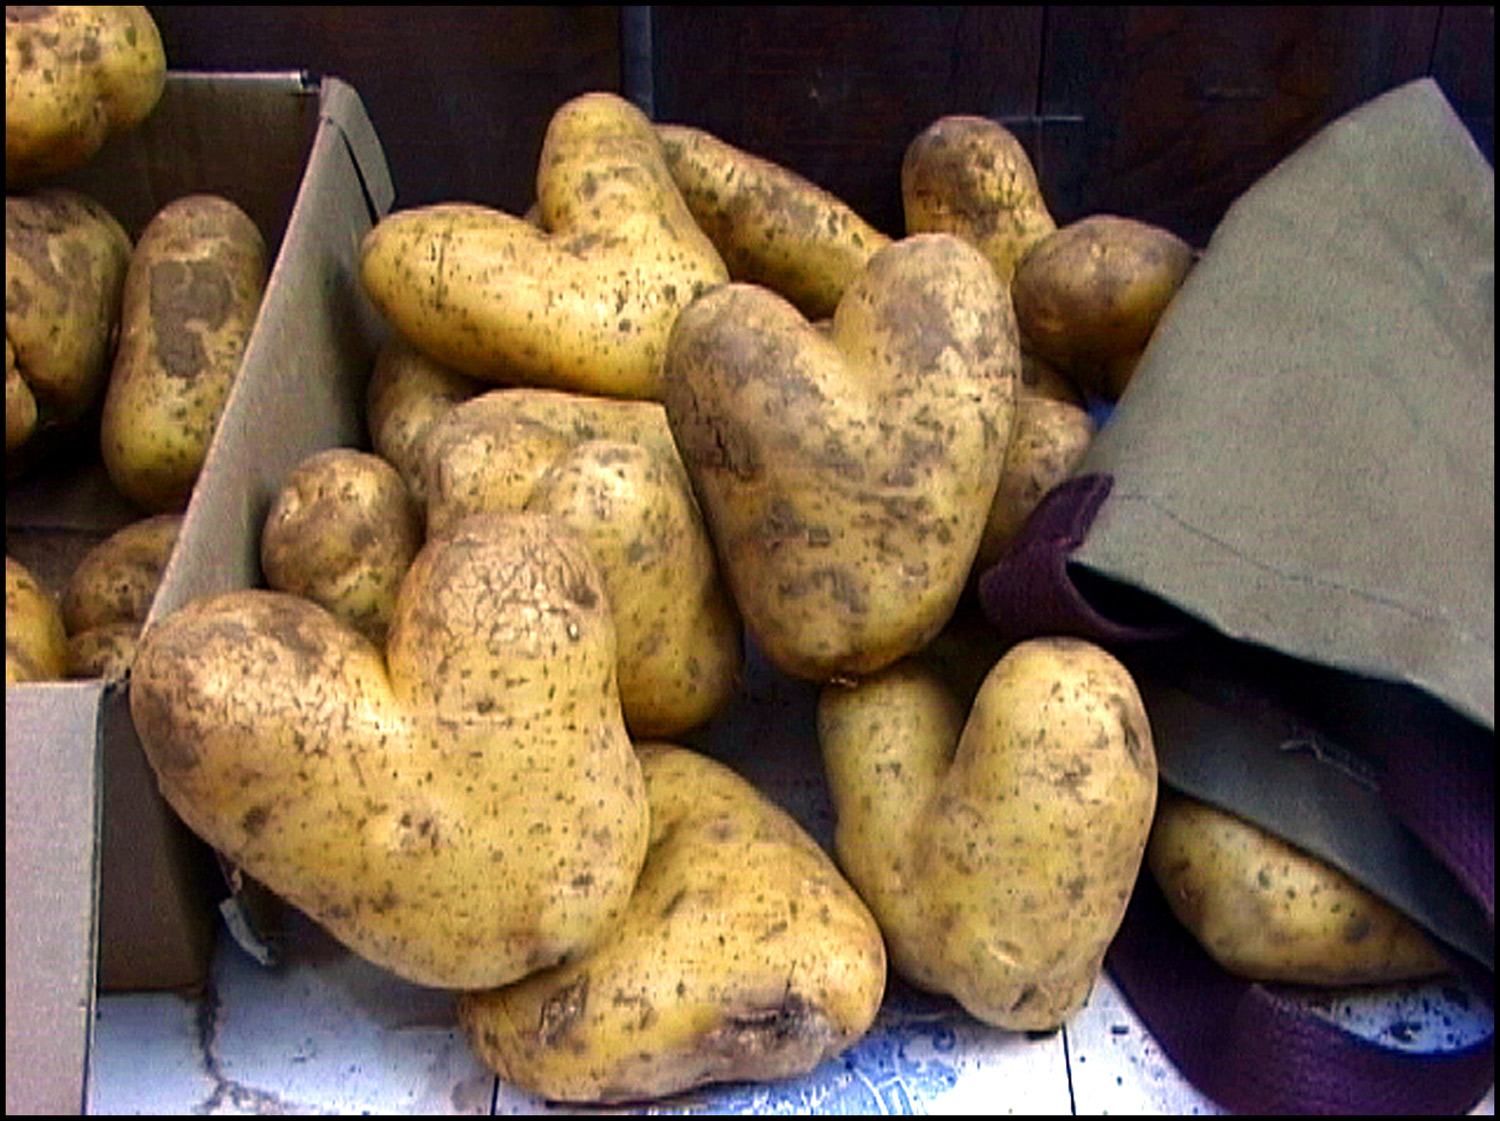
\includegraphics[height=6cm]{graphics/AgnesVarda_Potatoes.jpg}
  \caption{Still image from The Gleaners and I}
  \label{fig:AgnesVarda_Potatoes}
\end{figure}

The industrial processes have some standards and beyond that standards, there is not a place for anything. It clears out (or move away) the rest. It can be viewed as the idealization of goods and products (even people). At this point, it can be referred back to Žižek's claim that people's false consciousness about balanced and idealized notion of nature. It can be understood that this type of clarification of objects may result in this false perception. What Varda's finding is an excellent exemplification of what Žižek wants to point out.

Contrary to the common act of discarding, Varda finds out a creative way to use her unconscious recorded piece that might be deleted by the others. It is the scene where Varda had forgotten to turn her camera off and accidentally films the ground and her lens cap bouncing along as she walks. She uses this scene with a jazz soundtrack at background. Watching this scene is confusing at first hand regarding context. It might be viewed as worthless and recorded by accident. One can ask that why is this placed here, what does this have to do with gleaning? However, Varda forces us to watch it (wants us to pay attention). This scene called "the dance of the lens cap". Ruth Cruickshank in the article, The Work of Art in the Age of Global Consumption: Agnes Varda’s Les Glaneurs et la glaneuse (The Gleaners and I), addressed this scene and clarified the potential deeper meaning behind it. Cruickshank likened the scene to something that is normally thrown away, or in this case edited out of the film, much like the way trash is thrown away or food is left behind after a harvest. \quotes{Where many documentary makers would leave such accidental footage on the cutting room floor, Varda draws attention to how what would habitually be perceived as waste may be viewed as supplement with its own intrinsic value. Rather than literally treating it like dirt, Varda retains and prompts reassessment of that which is normally left out of shot} \cite{cruickshank2007work}. Things that are often forgotten or discarded can easily be revamped to create something useful to someone. The scene was revamped using music, and it became beautiful, much like the gleaners who found fish in the trash cooked it to make it edible, or the artist gleaner who piled discarded baby dolls into totem poles.

\todo{image}

As Varda demonstrates, people can be discovered throughout the French countryside gleaning everything from potatoes to grapes, apples to oysters, much as they did hundreds of years ago (though no longer in organized groups). Making use out of something that has been left behind and labeled as obsolete is not unique to potatoes. There is so much discarded, yet still-viable food in dumpsters that many people live off it entirely. More figuratively, there are also urban gleaners who salvage scraps from bins, appliances from the side of the road, or vegetables from stalls after the markets have closed. By showing them she shows that once was a common practice of gleaning throughout the years has evolved, but not disappeared. She keeps light to the modern life gleaners that are not visible every time. One of the is the teacher named Alain, an urban gleaner with a master's degree who teaches French to immigrants. Probably he has all the capabilities that live amoung the other people(???). It can seen that from this example, gleaning becomes also a form of resistence to ruling system. a way of refusing to be boxed in by conventional expectations

\todo{waste and want rules of eating from garbage.}

She shows that the act of gleaning does not bound to the collecting food and survival reasons. Some of them build their own meaning and existig and identity through the collected items. One of the examples that she gaves is ghat the man who collects baby dolls and use them in the decoration of his home. Every where is filled up with the babydolls even if wall of the garden.

Through the film she experiences the act of gleaning with different people. At one side she gleans potatoes in the field and on the other side follows a man with biycle look for the garbages front of the homes. By documenting their life in action she also participate them. But she bring them her own perception to them. For example in the case of potato gleaning she collect the heart shaped ones which are attract attion of her. Moreover in the case of night searching, she finds a clock without hand. It has fullfiled lits function and leaved away. Most important part of clock is missing therefore it is not functioning. However for it is a different meaning. Not every time people seek that want to aware of time sometimes they wantto forget that. They want to challange them.

A clock without hands found the garbage pile and taken by Agnès Varda. It does not work properly but it has important meaning for her. The time does not go on and it does not remind her that she is aging. One of the interesting thing is here Agnès Varda feels that as a aging person will later become discarded person.

She talks and investigates artist that are using discarded items in the artworks. What people not found anything the artist see countless possibilities from them. There is always alternative ways to see something different. Giving life or finding life from discarded life. 

Here another point is that Agnes display images of people picking up things from the ground like their ancestors. Everyone somehow collecting things in their life but particularly she selects these people and their images in action. There should reason for this? For some individuals, gleaning is not a novelty or a clever way to save money, but a necessity of life. They require it to sustain their life. Combine the elements from different peoples that seems totally unrelated gains powerful theme for the documentary. What gleaning means become more open (or powerful). It draws a picture of body combination of different parts (connected, dependent to the each other). The reason of gleaning varies but the fact that gleaning is continues in different forms.

She discusses the importance found in the meaning and purpose of art forms like this: \quotes{Varda seeks to encourage viewers to consider what potential agency is demonstrated in the artfulness and contingency of gleaning by individuals excluded\ldots from the homogenizing systems of global consumption} \cite{cruickshank2007work}. One can find more treasure in trash than many of New York’s finest galleries and art exhibits; they bring a grassroots feel to what has always been seen as a stuffy and prude aspect of society.

Varda's other subjects include artists who incorporate discarded materials into their work, symbols she discovers during her filming, and the French laws regarding gleaning versus abandoned property. Varda also spends time with Louis Pons, who explains how junk is a "cluster of possibilities." Louis Pons (born 1927) is a French collage artist. He specializes in reliefs and assemblages made entirely from discarded objects and junk. In Agnès Varda's documentary The Gleaners and I, Pons explains his artistic process and understanding of art; what others see as "a cluster of junk," he sees as "a cluster of possibilities;" and that the function of art is to tidy up one's inner and exterior worlds.







%%%
%%%
%%%
%\section{Summary}

% FROM drink UP, author: Werthan, Sarah, artist: Leech, Gwyneth. A Year in Cups. http://gwynethleech.com/
% trash and art collided. Paper and art, actually paper already medium of art, but is there anything different here. Itself is a part of a work, not the drawing, or painting.
% Documenting via a blog or a website. (what type of dimension it brings the work? maybe connect them, leave message.)
% Buying a beverage is a daily event for \ldots
% Creating art in public places can demystify the process for passers by, Leech says, making artistic expression more accessible and part of people’s everyday lives. The reason of website.
% “People see that an artist can make work anywhere, and make creative spaces anywhere,” she asserts. 


% TODO PRAP. from rethink, reimagine, reinvent
%\paraphrase{Recycling art approach to using reclaimed objects in artworks requires rethinking, or examining the affordances of a particular object to explore the possibilities for the object's inclusion in an artwork. Assemblage art involves the creation of new and innovative objects from what were once considered objects of waste; that is. through their use in assemblage pieces, reclaimed objects are endowed with a new. sometimes paradoxical meaning. The transformations of the objects used in assemblage pieces ask viewers to reconsider the notion of "valuable" as they are challenged to look at everyday objects with a new perspective (Taylor, 2006). Viewers confront issues relating to the functionality of objects during modern processes of production, consumption and distribution.}





%"Garbage art (alternatively known as trash art or recycled art) is art created from materials including post-consumer and other waste, collected debris, or objects previously used for other purposes." "Creating art from garbage involves transforming the meaning of objects by placing them in new, aestheticized contexts. This practice is not new; tribal peoples have adapted bits of trash from industrialized societies into their traditional arts since coming into contact with products of the developed world." "Creating art from trash involves “consuming” garbage in the sense that artists appropriate and rearrange the materials in personal ways, transform their meanings, utilize them to their own ends, and represent them in new ways.It involves taking unwanted materials out of their “waste” context and recontextualizing them as “art.”" \cite{tauxe2012encyclopedia}





%
%
%\textbf{What might be the meaning of using trash as a medium in the artworks? Questioning trash as a medium for artist}
%\begin{itemize}
%\item Some works try to raise awareness the problems that are the result of trash. (It treats environment and nature.)
%\item Some of them reflect people's lifestyle especially throw away culture. As a mirror of current lifestyle.
%\item Try to find a new value and meaning from the discarded material that are useless anymore. To explore a new approach, new way. Subvert people's ideas about trash and their attitudes by turning materials to the something meaningful (or valuable). Trash to treasure.
%\item Using discarded item to represent other discarded things by the ruling ideology or approach. For example, trash can be used to represent refugees. The things that we are trying to discard does not mean that they have no value, instead it means that we have no ability to reveal its potential. In other words, refugees have potential but we see them as players that will change our current system. Therefore, it can be said that willing to transform trash to treasure is to require change of current lifestyle. Rejecting discarding something especially thing that you get value from it is a process and spread through to the ones life.
%\item One way is not to produce trash. (Zero trash philosophy.) The other one is to transform trash into something else.
%\item What type of experience is that collecting and working on objects that are generally discarded? Experiencing out of common practice, being open to new explorations.
%\item Instead of a world that produce trash, how could it be a world created from trash?
%\item Combining industrial goods with objects transformed from trash is another way to find a place to trash in the community. It also signifies that trash still has a good quality to used with new materials. Creating composite products from new and reused items. Using the valuable thing with the invaluable thing. It becomes more valuable or less valuable. Depends on the perception.
%\item Aesthetics of trash. Revealing aesthetics value of discarded stuff. (Unique visual value. Trash portraits, sculptures etc.)
%\end{itemize}











% Sanatsal bir eylem olduğuna nasıl varacağım peki? Çünkü topluyorsun, belli bir yaklaşım geliştiriyorsun. Bu eyleme insanları davet ediyorsun. Sanatın eylem olma olayı... Buna burda değinip, kendi işime geçmeliyim.

% TODO 4th chapter
% Childs can enjoy with trash. I remember from my childhood, we collect crown cap and play with them. Some caps are found less and they worth more. We are looking everywhere for them. To make them flat we put them on the railways. After train passed we get perfect plat cap. At that time it is not trash for us. It has a value and part of our games and enjoy. To have fun a bunch of trash can be enough for us.

% TODO From Beautiful Trash Art and Transformation BY PAOLA IBARRA, ReVista
%Recycling has always been a common practice in the arts at least at a non-material level. From creating a world of words in literature, to rhythm and images in poetry, sampling in hip hop music, representation in the visual arts, or editing the illusory continuity of a film, art implies taking disparate elements (ideas, images, references, objects, etc.) and putting them together to form a new whole. Take and put. De-contextualize and re-contextualize. In that sense, art, as a system, is an act of recycling [from PAOLA IBARRA]. 

% TODO new comer
% FROM Book: Recycled, Re-Seen: Folk Art from the Global Scrap Heap
%\summary{Resistance} 
%\comment{Resistance, tactile, agnes varda?} If it is ultimately romantic to speak of these toys (or any other modern-day recyclia) in the language of resistance (by which I mean self-conscious political opposition), I would agree with Marshal Sahlins's assertion that "whether or not it comes to this [resistance], the indigenous mode of response to imperialism is always culturally subversive, insofar as the people must need to interpret the experience and they can do so only according to their own principles of existence. (sahlins 1992, 16)"

% TODO new comer
% FROM Book: Recycled, Re-Seen: Folk Art from the Global Scrap Heap
%\summary{Ironic}
%\comment{IRONIC, maybe added to results of transformation, reusing trashed items in different contexts.} This misuse the detritus of the industrial age has been described by western theorist as ironic. the irony is often embodied visually and conceptually. opposite of natural use, expected perception. for example making something from nothing or turning trash into treasure. By juxtaposing different materials changing context and place. 

% TODO new comer
% FROM Book: Recycled, Re-Seen: Folk Art from the Global Scrap Heap
%\comment{People applies their own perception to interpreted the items.} Human manufactured never envisioned possibilities seen by people. It suggests a self-confididence and intellectual authority that allows local peoples to encompass western goods in their own meanings "in their own scheme of things." 